\documentclass[13pt, aspectratio=169]{beamer}
\setbeamertemplate{navigation symbols}{}
\usepackage{fontspec}
\setsansfont{Calibri}
\AtBeginSection[]{
\begin{frame}
	\vfill
	\centering
	\begin{beamercolorbox}[sep=8pt,center,shadow=true,rounded=true]{title}
		\usebeamerfont{title}\insertsectionhead\par%
	\end{beamercolorbox}
	\vfill
\end{frame}
}
% \usepackage{silence}
% \WarningsOff[everypage]% Suppress warnings related to package everypage
% \WarningsOff
\usepackage{array}
\usepackage{url}
\usepackage{booktabs}
% \usepackage[]{tabularx}
\usepackage{amssymb}
\usepackage{amsthm}
\usepackage{tikz}
\usepackage{array}
\usepackage{booktabs}
\usepackage[]{tabularx, graphicx}
\graphicspath{{pictures/}}
% \usepackage{background}
\usepackage{parskip}
% \usepackage[absolute,overlay]{textpos}
\usepackage{xcolor}
% \usepackage{lipsum}
\usepackage{wrapfig}
\usepackage{tabularx,colortbl}
\usepackage{hyperref}
\usepackage{lipsum}

\title{Web Application Security}
\subtitle[]{Part 2}
\author{Sivasubramanian Natarajan}
\institute{Presented at SNU}
\date{Updated 3 Feb 2026}
\setbeamertemplate{footline}[frame number]

\setbeamercolor{itemize item}{fg=red}
\setbeamercolor{itemize subitem}{fg=red}
\setbeamercolor{itemize subsubitem}{fg=blue}

\setbeamertemplate{itemize item}[square]
\setbeamertemplate{itemize subitem}[circle]
\setbeamertemplate{itemize subsubitem}[circle]

\setbeamertemplate{footline}[text line]{%
\parbox{\linewidth}{\centering
Web Application Security CS4013 \hfill
\insertshortauthor \hfill
\insertframenumber{} / \inserttotalframenumber} }
% Source - https://tex.stackexchange.com/a/59131
% Posted by mbork
\setlength{\emergencystretch}{3pt}
% Retrieved 2026-03-24, License - CC BY-SA 3.0

\begin{document}
\begin{frame}


\includegraphics[width=.9\textwidth] {ssnlogo.png}

\end{frame}

% Section Page

 \begin{frame}
\frametitle{}
\fontsize{14pt}{12pt}\selectfont
\begin{columns}
\begin{column}{0.3\textwidth}
\begin{tabular}{l}
Web Application Security\\
\end{tabular}
\end{column}
\vrule
\begin{column}{0.5\textwidth}
\begin{tabular}{l}
Part 5 \\
\midrule
Updated Aug 6, 2026 \\
\midrule
Presented at SNU Chennai \\
\midrule
Sivasubramanian Natarajan
\end{tabular}
\end{column}
\end{columns}
\end{frame}

\begin{frame}
\frametitle{Recommended Text books}
\begin{itemize}
\item Web Application Security, Andrew Hoffman (O'Reilly)
\item Grokking Web application security, Malcom Macdonald (Manning Books)
\end{itemize}
\end{frame}


\section{Recap}

\begin{frame}
\frametitle{Previous class Summary}
\begin{itemize}
  \item Structure of a web application
  \item Threat Model (DFD, Trust Boundary, Strength/Weakness/Countermeasure)
  \item Threat Intelligence Platform operations
  \item Roadmap for the course
  \item Leveraging MITRE ATT\&CK Framework
\end{itemize}
\end{frame}

\section{Hacking Web applications}

\begin{frame}
\frametitle{Cross site Scripting data flow}
\small \url{https://portswigger.net/web-security/cross-site-scripting} 
\centering 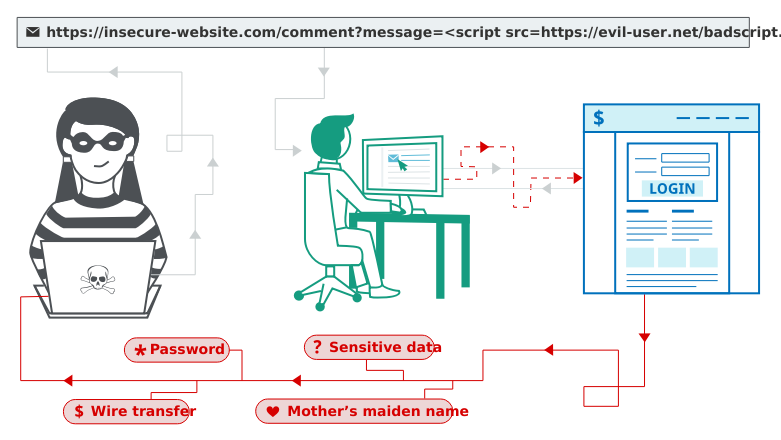
\includegraphics[width=.9\textwidth] {xss.png}
\end{frame}

\begin{frame}
	\frametitle{Cross site Scripting XSS}
	Below is a classification of XSS
	\begin{itemize}
		\item Stored XSS
		\item Reflected XSS
		\item DOM XSS
	\end{itemize}
\end{frame}

\begin{frame}
	\frametitle{Reflected XSS}
\begin{itemize}
	\item Reflected attacks are those where the injected script is reflected off the web server, such as in an error message, search result, or any other response that includes some or all of the input sent to the server as part of the request. 
	\item It could be embedded in an email link or something the user clicks on the website inadvertently.
\end{itemize}
	
\end{frame}

\begin{frame}
	\frametitle{Stored XSS}
\begin{itemize}
	\item Stored attacks are those where the injected script is permanently stored on the target servers, such as in a database, in a message forum, visitor log, comment field, etc. 
	\item The victim then retrieves the malicious script from the server when it requests the stored information. 
	\item Stored XSS is also sometimes referred to as Persistent or Type-II XSS.
\end{itemize}
	
\end{frame}

\begin{frame}
\frametitle{DOM XSS}

\begin{itemize}
	\item DOM Based XSS (or as it is called in some texts, “type-0 XSS”) is an XSS attack wherein the attack payload is executed as a result of modifying the DOM “environment” in the victim’s browser used by the original client side script, so that the client side code runs in an “unexpected” manner. 
	\item That is, the page itself (the HTTP response that is) does not change, but the client side code contained in the page executes differently due to the malicious modifications that have occurred in the DOM environment.
\end{itemize}
	
\end{frame}

\begin{frame}
	\frametitle{Case Study XSS attack}
Reference: MITRE : Enterprise Matrice, Tactic: Initial Access, Technique: Drive by compromise
	\begin{itemize}
		\item Adversaries may gain access to a system through a user visiting a website over the normal course of browsing. 		
		\item A legitimate website is compromised, allowing adversaries to inject malicious code
		\item Malicious ads are paid for and served through legitimate ad providers (i.e., Malvertising)
		\item Built-in web application interfaces that allow user-controllable content are leveraged for the insertion of malicious scripts or iFrames (e.g., cross-site scripting)
	\end{itemize}
\url{https://attack.mitre.org/techniques/T1189/}

\end{frame}

\begin{frame}
	\frametitle{APT 28}
Reference:\\ \small \url{https://blog.google/threat-analysis-group/ukraine-remains-russias-biggest-cyber-focus-in-2023/}

\begin{itemize}
	\item Refer section: FROZENLAKE uses XSS in phishing against Ukranian users
	\item In early 2023, another Russian GRU actor TAG tracks as FROZENLAKE (aka APT28) was especially focused on Ukraine. In February and March, they sent multiple large waves of phishing emails to hundreds of users in Ukraine, continuing the group’s 2022 focus on targeting webmail users in Eastern Europe.
	
	\item Starting in early February 2023 we saw FROZENLAKE using reflected cross-site scripting (XSS) on multiple Ukrainian government websites to redirect users to phishing pages - a new TTP for the group. 
	\end{itemize}

\end{frame}

\begin{frame}
	\frametitle{Hacker Motives}
	
	\begin{itemize}
		\item Impersonate or masquerade as the victim user.
		\item Read any data that the user is able to access.
		\item Capture the user's login credentials.
	\end{itemize}
\end{frame}



\begin{frame}
\frametitle{Detection}
\url{https://attack.mitre.org/detectionstrategies/DET0176/\#AN0501}	\\
\begin{itemize}
	\item Manually testing for reflected and stored XSS normally involves submitting some simple unique input (such as a short alphanumeric string) into every entry point in the application, identifying every location where the submitted input is returned in HTTP responses, and testing each location individually to determine whether suitably crafted input can be used to execute arbitrary JavaScript.  
	\item In this way, you can determine the context in which the XSS occurs and select a suitable payload to exploit it.
	\item Manual testing can be extremely time-consuming. Burp Suite's web vulnerability scanner combines static and dynamic analysis of JavaScript to reliably automate the detection of DOM-based vulnerabilities. 
\end{itemize}
\end{frame}
	
\begin{frame}
	\frametitle{Mitigation / Countermeasure}
	\begin{itemize}
		\item Content Security Policy
		\item Class discussion \url{https://blogs.windows.com/msedgedev/2017/03/23/strengthening-microsoft-edge-sandbox/}
	\end{itemize}
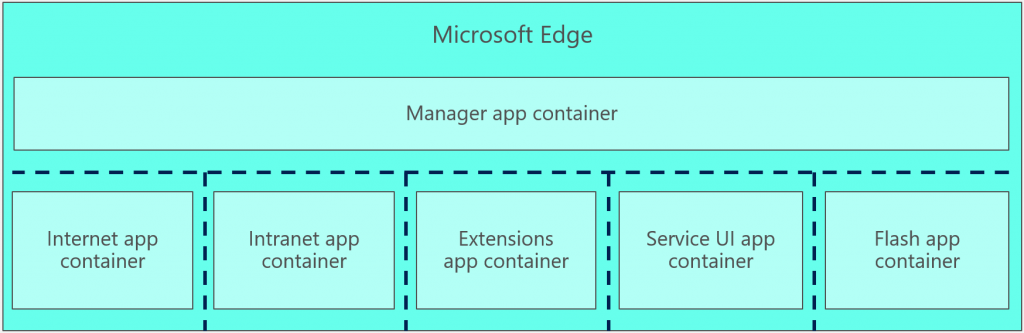
\includegraphics[width=\textwidth]{edge-appcontainer.png}
\end{frame}

\end{document}


